%%
%% DCBA: Dual-Chain Blockchain Architecture for Secure,
%% Priority-Aware, UAV-Enabled Pharmaceutical Delivery
%% ACM SIGPLAN Proceedings Template
%%
%% For review: use \documentclass[sigplan,review,anonymous]{acmart}
%% For submission: use \documentclass[sigplan,screen]{acmart}
%%
\documentclass[sigplan,screen]{acmart}

%% ─── ACM Rights ────────────────────────────────────────────────
\setcopyright{rightsretained}
\copyrightyear{2026}
\acmYear{2026}
\acmDOI{XXXXXXX.XXXXXXX}
\acmConference[PLACEHOLDER]{Name of Conference}{Month DD--DD, Year}{City, Country}
\acmISBN{978-1-4503-XXXX-X/26/XX}

%% ─── Packages ──────────────────────────────────────────────────
\usepackage{algorithm}
\usepackage{algpseudocode}
\usepackage{booktabs}
\usepackage{multirow}
\usepackage{xspace}
\usepackage{balance}
\usepackage{listings}
\usepackage{pgfplots}
\usepackage{tikz}
\usetikzlibrary{shapes.geometric, arrows.meta, positioning, fit, backgrounds,
                decorations.pathreplacing, calc}
\pgfplotsset{compat=1.18}
\usepackage{microtype}
\usepackage{amsmath}
\usepackage{amssymb}
\usepackage{graphicx}

%% ─── Custom commands ───────────────────────────────────────────
\newcommand{\dcba}{\textsc{DCBA}\xspace}
\newcommand{\pdc}{PDC\xspace}
\newcommand{\uoc}{UOC\xspace}
\newcommand{\dcs}{\textsc{DCS}\xspace}
\newcommand{\pars}{\textsc{PARS}\xspace}
\newcommand{\rxhash}{\texttt{rxHash}\xspace}
\newcommand{\mblock}{\textsc{MBlock}\xspace}
\newcommand{\upremium}{$\upsilon_{\text{premium}}$\xspace}
\newcommand{\unormal}{$\upsilon_{\text{normal}}$\xspace}
\newcommand{\etal}{\textit{et al.}\xspace}

%% Solidity listings style
\lstdefinelanguage{Solidity}{
  keywords={pragma, solidity, contract, function, public, private,
            mapping, address, uint256, uint8, bool, string, bytes32,
            struct, enum, event, emit, require, returns, view, pure,
            modifier, constructor, memory, storage, external, internal,
            if, else, for, return, new, delete, true, false, msg, block},
  keywordstyle=\bfseries\color[HTML]{2563EB},
  commentstyle=\itshape\color[HTML]{4B5563},
  stringstyle=\color[HTML]{059669},
  basicstyle=\ttfamily\footnotesize,
  frame=single, numbers=left, numberstyle=\tiny\color{gray},
  breaklines=true, tabsize=2, showstringspaces=false
}

%% ─── TikZ styles ───────────────────────────────────────────────
\tikzset{
  actor/.style={draw, rectangle, rounded corners=3pt,
    minimum width=2.0cm, minimum height=0.55cm,
    font=\footnotesize\bfseries, align=center},
  sc/.style={draw, ellipse, minimum width=1.8cm, minimum height=0.5cm,
    font=\footnotesize, align=center},
  chain/.style={draw, rectangle, rounded corners=6pt,
    minimum width=5.2cm, dashed, thick},
  arr/.style={-Stealth, thick},
  darr/.style={-Stealth, dashed, thick},
  flow/.style={draw, rectangle, rounded corners=2pt,
    minimum width=2.6cm, minimum height=0.5cm, font=\footnotesize, align=center},
  decision/.style={draw, diamond, aspect=2.2,
    minimum width=2.2cm, minimum height=0.5cm, font=\scriptsize, align=center},
  fstart/.style={draw, circle, fill=black, minimum size=0.22cm},
  fend/.style={draw, circle, fill=black, minimum size=0.18cm,
    double, double distance=1.5pt}
}

%% ───────────────────────────────────────────────────────────────
\begin{document}

\title{\dcba: A Dual-Chain Blockchain Architecture for Secure,\\
       Priority-Aware, UAV-Enabled Pharmaceutical Delivery}

\author{Ankan Saha}
\affiliation{
  \institution{Department of Computer Science and Engineering}
  \institution{Bangladesh University of Engineering and Technology (BUET)}
  \city{Dhaka}
  \country{Bangladesh}
}
\email{ankan@student.buet.ac.bd}

%% Add co-authors here if applicable
%% \author{Author Two}
%% \affiliation{...}

\renewcommand{\shortauthors}{Saha}

%% ─── Abstract ──────────────────────────────────────────────────
\begin{abstract}
Pharmaceutical supply chain fraud — responsible for an estimated one million deaths
annually — and last-mile delivery failure in high-density urban environments define
two converging crises that no existing blockchain or UAV system jointly addresses.
We present \dcba (\textbf{D}ual-\textbf{C}hain \textbf{B}lockchain
\textbf{A}rchitecture), a system that integrates a patient-private Ethereum
Proof-of-Authority chain (\pdc) with an IoT-optimised Hyperledger~Fabric chain
(\uoc) to enforce prescription integrity, patient data sovereignty, and
priority-aware drone delivery in a single cohesive architecture.
\dcba introduces six original contributions: a purpose-separated dual-chain
design; hardware-bound W3C Decentralised Identifiers (DIDs) for UAVs; a
two-phase Drone Capability Score (\dcs) algorithm using Bloom-filter
pre-screening and ECDSA verification; sanitisable-signature medical records;
a four-tier Priority-Aware Routing System (\pars) with on-chain SLA
enforcement; and patient-sovereign asymmetric encryption.
Experimental evaluation over 86 automated tests and Hyperledger Caliper
benchmarking demonstrates 100\% security-test pass rate, DCS selection in
8.37\,ms for 100~UAVs ($16.7\times$ below target), zero replay attacks
accepted, and zero delivery confirmation or deviation failures.
\end{abstract}

\begin{CCSXML}
<ccs2012>
  <concept>
    <concept_id>10002978.10003006.10011634</concept_id>
    <concept_desc>Security and privacy~Distributed systems security</concept_desc>
    <concept_significance>500</concept_significance>
  </concept>
  <concept>
    <concept_id>10002978.10002986</concept_id>
    <concept_desc>Security and privacy~Cryptography</concept_desc>
    <concept_significance>300</concept_significance>
  </concept>
  <concept>
    <concept_id>10010147.10010257</concept_id>
    <concept_desc>Computing methodologies~Distributed computing methodologies</concept_desc>
    <concept_significance>300</concept_significance>
  </concept>
</ccs2012>
\end{CCSXML}
\ccsdesc[500]{Security and privacy~Distributed systems security}
\ccsdesc[300]{Security and privacy~Cryptography}
\ccsdesc[300]{Computing methodologies~Distributed computing methodologies}

\keywords{blockchain, dual-chain architecture, pharmaceutical delivery, UAV,
  smart contracts, W3C DID, Hyperledger Fabric, Ethereum PoA, Bloom filter,
  priority routing, SLA enforcement}

\maketitle

%%====================================================================
\section{Introduction}\label{sec:intro}
%%====================================================================

The World Health Organisation estimates that 10\% of medicines in
low-and-middle-income countries are substandard or falsified, causing roughly
one million deaths per year~\cite{who2017falsified}.
The problem is systemic: pharmaceutical supply chains span dozens of
intermediaries, and the paper-based, centralised record-keeping that governs
most dispensation workflows offers no tamper-evident audit trail.
In Bangladesh — the motivating deployment context for this work — the
Directorate General of Drug Administration (DGDA) oversees more than 257
licensed manufacturers yet lacks cryptographically enforceable traceability
from prescription to patient.

Simultaneously, last-mile delivery of time-critical medications is failing.
Dhaka's urban population density exceeds 44,000 persons per km²~\cite{bbs2022census},
and road-traffic paralysis makes conventional ground delivery unable to meet
the response windows that life-critical medications demand:
insulin for hypoglycaemia, epinephrine for anaphylaxis, or anticoagulants
for acute stroke must arrive in minutes.
Unmanned Aerial Vehicles (UAVs) have demonstrated clinical viability
for last-mile medical delivery~\cite{zipline2022lancet,thiels2015uav},
but existing deployments are centralised, proprietary, and entirely absent
from any blockchain-based accountability framework.

Blockchain technology offers immutability and decentralised trust, yet
deploying a single chain for both use cases creates an irreconcilable conflict:
patient health records demand privacy, controlled access, and permissioned
visibility; UAV operational data demands high throughput, IoT-grade latency,
and multi-organisational endorsement semantics.
No existing system reconciles these two requirement sets within a single
architecture while also providing provable UAV selection fairness, clinical
priority routing, and patient data sovereignty.

This paper presents \dcba (\textbf{D}ual-\textbf{C}hain
\textbf{B}lockchain \textbf{A}rchitecture), which resolves this conflict by
purpose-separating the two concerns onto two distinct chains connected by
a replay-safe cross-chain oracle.
Our contributions are:

\begin{itemize}
\item[\textbf{C1.}] A \emph{dual-chain architecture} pairing an Ethereum PoA
  Patient Data Chain (\pdc) with a Hyperledger Fabric UAV Operational Chain
  (\uoc), each optimised for its domain's privacy and performance requirements.

\item[\textbf{C2.}] \emph{Hardware-bound W3C DID identity} for UAVs via
  $h^\circ = H(\text{mac} \,\|\, \tau_s \,\|\, \text{seed})$, making device
  identity non-transferable and clone-resistant.

\item[\textbf{C3.}] A \emph{two-phase Drone Capability Score (\dcs) algorithm}
  combining Bloom-filter O(1) pre-screening with ECDSA verification to select
  $\upsilon_{\text{premium}}$ from a 100-UAV fleet in 8.37\,ms.

\item[\textbf{C4.}] \emph{Sanitisable-signature medical records} that preserve
  the Trusted Authority's root attestation while permitting authorised physician
  amendments within patient-consented bounds.

\item[\textbf{C5.}] A \emph{Priority-Aware Routing System (\pars)} with four
  clinically grounded urgency tiers and on-chain SLA deadlines enforced by
  smart contract, with anomaly detection for priority inflation.

\item[\textbf{C6.}] \emph{Patient-sovereign asymmetric encryption}: medical
  records are encrypted off-chain with the patient's public key before IPFS
  upload; only the patient's private key can decrypt them.
\end{itemize}

%%====================================================================
\section{Background and Related Work}\label{sec:related}
%%====================================================================

\subsection{Blockchain for Pharmaceutical Records}

MedRec~\cite{azaria2016medrec} pioneered smart-contract-based EHR access
control on Ethereum, but operated on a single public chain with no UAV
integration.
Sylim \etal~\cite{sylim2018blockchain} applied Hyperledger Fabric to
drug-supply monitoring, achieving provenance tracking but without patient
privacy guarantees — all channel participants can read records.
PharmaChain~\cite{pharmachain2023} and Jamil \etal~\cite{jamil2019novel}
extended Fabric-based drug traceability to smart hospital contexts, yet both
remain single-chain designs incompatible with the divergent throughput
and privacy demands of a combined prescription-and-delivery pipeline.

\subsection{UAV-Based Medical Delivery}

Zipline's Rwanda deployment~\cite{zipline2022lancet} demonstrated 12 million
drone deliveries with a 67\% reduction in blood-product wastage, establishing
clinical viability.
Thiels \etal~\cite{thiels2015uav} showed UAVs reach cardiac-arrest sites
materially faster than ambulances.
Task-allocation literature~\cite{skaltsis2023review} proposes auction
algorithms, PSO variants, and Hungarian-method approaches for multi-UAV
assignment, but none combines capability scoring with cryptographic
identity verification or Bloom-filter acceleration on a blockchain.

\subsection{Cross-Chain and Multi-Chain Architectures}

Belchior \etal~\cite{belchior2021survey} systematically classified 404
cross-chain protocols into public connectors, blockchain-of-blockchains, and
hybrid connectors, establishing that correct cross-chain communication requires
a trusted relay when the two chains share no state.
Hyperledger FireFly and Polkadot provide general-purpose cross-chain
infrastructure but impose no application-layer pharmaceutical semantics.
A recent dual-blockchain IoT healthcare paper~\cite{mallick2025dualchain}
separates public and private chains yet addresses neither UAV delivery, UAV
identity, nor priority-based SLA routing.

\subsection{Confirmed Research Gaps}
\label{subsec:gaps}

Table~\ref{tab:gaps} maps the six gaps that motivate \dcba.
The defining absence in the literature is any system that simultaneously
provides (i)~purpose-separated dual-chain architecture,
(ii)~hardware-bound UAV identity, (iii)~cross-chain prescription
verification, (iv)~encrypted capability scoring, (v)~on-chain clinical
priority routing, and (vi)~patient-sovereign encryption.

\begin{table}[t]
\caption{Research gaps addressed by \dcba.}
\label{tab:gaps}
\small
\begin{tabular}{@{}lp{4.6cm}@{}}
\toprule
\textbf{Gap} & \textbf{Description} \\
\midrule
G1 & No dual-chain architecture separating patient data from UAV operations \\
G2 & No hardware-bound UAV identity preventing cloning/impersonation \\
G3 & No replay-safe cross-chain prescription oracle for drug delivery \\
G4 & No encrypted UAV capability scoring with cryptographic verification \\
G5 & No on-chain clinical priority routing with SLA enforcement \\
G6 & No patient-sovereign encryption in blockchain EHR \\
\bottomrule
\end{tabular}
\end{table}

%%====================================================================
\section{System Architecture}\label{sec:arch}
%%====================================================================

\subsection{Design Principles}

\dcba is governed by three principles.
\textbf{Chain separation by purpose}: data with fundamentally different privacy
and throughput requirements must not coexist on the same ledger.
\textbf{Zero implicit trust}: every transaction requires explicit cryptographic
verification of actor identity, permission, and data integrity, regardless of
history or affiliation.
\textbf{Measurable accountability}: every significant event produces an
immutable, timestamped, cryptographically attributable record.

\subsection{Dual-Chain Overview}

Figure~\ref{fig:architecture} illustrates the \dcba architecture.

\begin{figure}[t]
\centering
\begin{tikzpicture}[node distance=1.3cm and 0.9cm, scale=0.82,
                    every node/.style={transform shape}]

%% ── PDC box ──────────────────────────────────────────────────────
\begin{scope}
\node[actor, fill=blue!8, draw=blue!60, text width=2.2cm] (sc1p)
      {SC-1\\Identity (PDC)};
\node[actor, fill=violet!8, draw=violet!60, text width=2.2cm,
      below=0.55 of sc1p] (sc2)
      {SC-2\\Consent};
\node[actor, fill=green!8, draw=green!60, text width=2.2cm,
      below=0.55 of sc2] (sc3)
      {SC-3\\Med Records};

\begin{pgfonlayer}{background}
\node[chain, draw=blue!50, fill=blue!3,
      fit=(sc1p)(sc2)(sc3),
      inner sep=6pt, label={[font=\footnotesize\bfseries, text=blue!70]above:
        PDC · Ethereum PoA}] (pdc) {};
\end{pgfonlayer}
\end{scope}

%% ── SC-7 oracle bridge ──────────────────────────────────────────
\node[actor, fill=amber!12, draw=orange!70, text width=2.1cm,
      right=1.5cm of sc2] (sc7)
      {SC-7\\Oracle Bridge};

%% ── UOC box ──────────────────────────────────────────────────────
\begin{scope}[xshift=5.8cm]
\node[actor, fill=blue!8, draw=blue!60, text width=2.2cm] (sc1u)
      {SC-1\\Identity (UOC)};
\node[actor, fill=amber!8, draw=orange!60, text width=2.2cm,
      below=0.55 of sc1u] (sc4)
      {SC-4\\DCS Scoring};
\node[actor, fill=violet!8, draw=violet!60, text width=2.2cm,
      below=0.55 of sc4] (sc5)
      {SC-5\\Delivery Orders};
\node[actor, fill=cyan!8, draw=cyan!60, text width=2.2cm,
      below=0.55 of sc5] (sc6)
      {SC-6\\Lifecycle};

\begin{pgfonlayer}{background}
\node[chain, draw=green!50, fill=green!3,
      fit=(sc1u)(sc4)(sc5)(sc6),
      inner sep=6pt, label={[font=\footnotesize\bfseries, text=green!70]above:
        UOC · Hyperledger Fabric}] (uoc) {};
\end{pgfonlayer}
\end{scope}

%% ── Actors (left) ───────────────────────────────────────────────
\node[actor, fill=gray!8, draw=gray!50, text width=1.5cm,
      left=1.2cm of sc1p] (pat) {Patient};
\node[actor, fill=gray!8, draw=gray!50, text width=1.5cm,
      left=1.2cm of sc3]  (hp)  {HP};

%% ── Actors (right) ──────────────────────────────────────────────
\node[actor, fill=gray!8, draw=gray!50, text width=1.5cm,
      right=1.2cm of sc4]  (uav) {UAV};
\node[actor, fill=gray!8, draw=gray!50, text width=1.5cm,
      right=1.2cm of sc5]  (ds)  {DS};
\node[actor, fill=gray!8, draw=gray!50, text width=1.5cm,
      right=1.2cm of sc6]  (dw)  {DW};

%% ── TA (top centre) ─────────────────────────────────────────────
\node[actor, fill=violet!12, draw=violet!70, text width=3.2cm,
      above=0.9cm of sc7]  (ta)
      {Trusted Authority (TA)};

%% ── Arrows ──────────────────────────────────────────────────────
\draw[arr, blue!60]  (pat) -- node[above,font=\tiny]{grant} (sc2);
\draw[arr, green!60] (hp)  -- node[above,font=\tiny]{addRecord} (sc3);
\draw[arr, orange!70](sc3) -- node[above,font=\tiny]{\tiny rxHash} (sc7);
\draw[arr, orange!70](sc7) -- node[above,font=\tiny]{\tiny verify} (sc5);
\draw[arr, cyan!60]  (uav) -- node[right,font=\tiny]{\tiny score} (sc4);
\draw[arr, cyan!60]  (uav) -- node[right,font=\tiny]{\tiny GPS} (sc6);
\draw[arr, green!60] (ds)  -- node[right,font=\tiny]{\tiny DCS} (sc4);
\draw[arr, orange!60](dw)  -- node[right,font=\tiny]{\tiny stock} (sc5);
\draw[darr,violet!70](ta)  -| (pdc);
\draw[darr,violet!70](ta)  -| (uoc);
\end{tikzpicture}
\caption{\dcba dual-chain architecture. Solid arrows show primary data flows;
  dashed arrows show TA governance. SC-7 is the cross-chain oracle bridge.}
\label{fig:architecture}
\end{figure}

\noindent
\textbf{\pdc} is an Ethereum Proof-of-Authority network running the Patient
Private Channel (PPC). It hosts SC-1 (identity), SC-2 (consent), SC-3
(medical records), and SC-7 (oracle bridge).
Block time is 2--5\,s; gas is waived in the permissioned environment.

\noindent
\textbf{\uoc} is a Hyperledger Fabric 2.5 Raft network hosting SC-1 (mirrored
identity), SC-4 (DCS scoring), SC-5 (delivery orders), and SC-6 (lifecycle).
It is optimised for high-frequency UAV telemetry and multi-organisational
endorsement.

\subsection{Principal Actors}

Eight actors participate in \dcba. Table~\ref{tab:actors} summarises their
chain access rights and primary cryptographic responsibilities.

\begin{table}[t]
\caption{Principal actors and their roles in \dcba.}
\label{tab:actors}
\small
\begin{tabular}{@{}p{1.5cm}p{1.2cm}p{3.5cm}@{}}
\toprule
\textbf{Actor} & \textbf{Chain} & \textbf{Key responsibilities} \\
\midrule
Trusted Authority (TA)
  & Both (admin) & Issues W3C DIDs; maintains SC-1 on both chains;
    enforces validator anti-collusion \\[2pt]
Patient
  & PDC light & Holds $\text{keypri}_P$; grants/revokes HP consent;
    confirms delivery \\[2pt]
Healthcare Provider (HP)
  & PDC full & Encrypts and signs \mblock; assigns \pars score;
    submits delivery orders \\[2pt]
Drug Warehouse (DW)
  & UOC full & Confirms stock; hands package to $\upsilon_{\text{premium}}$ \\[2pt]
Drone Station (DS)
  & UOC full & Opens/closes DCS rounds; holds $\text{keypri}_{DS}$;
    monitors GPS \\[2pt]
UAV
  & UOC IoT & Computes DCS; encrypts score; streams GPS to IPFS \\[2pt]
Miner / Validator
  & Both (infra) & PoA consensus (PDC); Fabric Raft endorsement (UOC) \\[2pt]
Regulatory Auditor (RA)
  & Both (read) & Audits \pars anomalies; generates DGDA reports \\
\bottomrule
\end{tabular}
\end{table}

\subsection{Smart Contract Summary}

\dcba deploys seven smart contracts.
On the \pdc, SC-1 registers and revokes every actor's DID; SC-2 manages
patient-issued time-limited consent tokens; SC-3 stores encrypted \mblock
references and atomically triggers SC-7 on every write; SC-7 maintains an
rxHash state machine (PENDING $\!\to\!$ VALID $\!\to\!$ USED) providing
replay-safe cross-chain prescription verification.
On the \uoc, SC-4 executes two-phase DCS scoring rounds; SC-5 manages the
\pars priority queue and calls the SC-7 oracle before creating any order;
SC-6 operates the delivery state machine and stores IPFS GPS hashes.

The deployment order is strictly: SC-1 $\to$ SC-7 $\to$ SC-2 $\to$ SC-3 $\to$
SC-4 $\to$ SC-5 $\to$ SC-6, with two mandatory post-deployment link calls:
\texttt{SC7.setSC3Address()} and \texttt{SC4.linkSC6()}.
These links enforce that only SC-3 may register prescription hashes in SC-7,
and only SC-6 may call \texttt{updateReputation()} in SC-4 without holding a
DID — preventing administrative substitution attacks.

%%====================================================================
\section{Core Mechanisms}\label{sec:mechanisms}
%%====================================================================

\subsection{Drone Capability Score (DCS)}
\label{subsec:dcs}

\subsubsection{Score Computation}
Each UAV computes its capability score $c_s \in [0,100]$ locally before
submission, using a weighted linear combination of five operational metrics:

\begin{equation}
  c_s = \frac{\omega_1 \nu_{\max} + \omega_2 \rho_{\text{cap}} +
             \omega_3 \beta_{\text{pow}} + \omega_4 C_{\text{pu}} +
             \omega_5 R_{\text{am}}}
            {100} + \sum_i \omega_i O_i
  \label{eq:dcs}
\end{equation}

\noindent where $\nu_{\max}$ is normalised maximum speed, $\rho_{\text{cap}}$
payload capacity, $\beta_{\text{pow}}$ battery level, $C_{\text{pu}}$ CPU
availability ($1 - \text{utilisation}$), and $R_{\text{am}}$ RAM availability;
$O_i$ are optional operational parameters.
The weights $\omega = (0.30,\, 0.25,\, 0.20,\, 0.15,\, 0.10)$ reflect
the relative importance of speed, payload, battery, CPU, and RAM for
pharmaceutical delivery, and sum to $1.0$.
\texttt{computeScore()} is declared \texttt{pure} in Solidity: UAVs call it
off-chain to avoid on-chain gas costs.

\subsubsection{Two-Phase Submission Protocol}
Raw scores are never submitted in plaintext.
Prior to submission each UAV:
(1)~encrypts $c_s$ for the Drone Station:
    $\varepsilon_s = \text{Enc}(c_s,\, \text{keypub}_{DS})$; and
(2)~signs the ciphertext:
    $\sigma = \text{Sign}(\varepsilon_s,\, \text{keypri}_{UAV})$.
The pair $(\varepsilon_s, \sigma)$ is submitted to SC-4.

\noindent\textbf{Phase~1 — Bloom Filter.}
SC-4 checks a 1024-bit Bloom filter (parameters: $n=100$, $\varepsilon=0.01$,
$k=7$, $m=959\,\text{b} \approx 1\,\text{kib}$).
Submissions whose DID hashes are absent from the filter are dropped in $O(1)$;
the false-negative rate is provably zero, so no registered UAV is ever
incorrectly rejected.

\noindent\textbf{Phase~2 — ECDSA Verification.}
For submissions that pass Phase~1, SC-4 retrieves \texttt{keypub\_UAV} from
SC-1 and verifies $\sigma$.
Only verified ciphertexts are decrypted by the DS using $\text{keypri}_{DS}$.
SC-4 then sorts plaintext scores and assigns
$\upsilon_{\text{premium}} = \arg\max(c_s)$.

Algorithm~\ref{alg:dcs} formalises the DCS protocol.

\begin{algorithm}[t]
\caption{Two-Phase DCS Selection}\label{alg:dcs}
\footnotesize
\begin{algorithmic}[1]
\Require Fleet $\mathcal{U} = \{u_1,\ldots,u_N\}$, Bloom filter $\mathcal{B}$,
         $\text{keypub}_{DS}$
\Ensure  Winner $u^*$, verified set $\mathcal{V}$
\State DS calls \texttt{SC4.openRound(orderId)} $\to$ roundId
\ForAll{$u_i \in \mathcal{U}$} \textbf{in parallel}
  \State $c_i \leftarrow \texttt{computeScore}(\nu,\rho,\beta,C,R)$
  \State $\varepsilon_i \leftarrow \text{Enc}(c_i,\, \text{keypub}_{DS})$
  \State $\sigma_i \leftarrow \text{Sign}(\varepsilon_i,\, \text{keypri}_{u_i})$
  \State Submit $(\varepsilon_i, \sigma_i)$ to \texttt{SC4.submitScore()}
\EndFor
\State \textbf{Phase 1:} $\mathcal{U}' \leftarrow \{u_i : \texttt{DID}(u_i) \in \mathcal{B}\}$
  \hfill\Comment{O(1) per UAV}
\State \textbf{Phase 2:} $\mathcal{V} \leftarrow \{u_i \in \mathcal{U}' : \texttt{Verify}(\varepsilon_i,\sigma_i,\text{keypub}_{u_i})\}$
\State DS decrypts: $c'_i \leftarrow \text{Dec}(\varepsilon_i, \text{keypri}_{DS})$ for $u_i \in \mathcal{V}$
\State DS calls \texttt{SC4.closeRound(roundId)}
\State $u^* \leftarrow \arg\max_{u_i \in \mathcal{V}}(c'_i)$
  \hfill\Comment{$\upsilon_{\text{premium}}$}
\end{algorithmic}
\end{algorithm}

\subsection{Priority-Aware Routing System (PARS)}
\label{subsec:pars}

\subsubsection{PARS Score Calculation}

The HP assigns a clinical priority score $P \in [0,100]$ at prescription
creation, following a structured four-factor rubric:

\begin{equation}
  P = \lfloor 100 \cdot I_u \cdot (1 + \alpha \cdot T_f + \beta \cdot R_f) \rfloor
  \label{eq:pars}
\end{equation}

\noindent where $I_u \in \{0.90,\, 0.75,\, 0.55,\, 0.30\}$ is the
\emph{clinical urgency indicator} derived from ICD-10 diagnosis severity
class (life-threatening / serious / routine / elective);
$T_f \in [0,1]$ is the \emph{therapeutic time-sensitivity factor},
computed as $1 - t_{\text{window}} / t_{\text{max}}$ where $t_{\text{window}}$
is the drug's critical administration window and $t_{\text{max}}$ a reference
normalisation constant (24\,h);
$R_f \in [0,1]$ is the \emph{route-delay penalty}, estimated from the
patient's location relative to the nearest Drug Warehouse
($R_f = \min(d/d_{\text{max}}, 1)$ where $d$ is road-distance);
and $\alpha=0.07$, $\beta=0.03$ are empirically tuned weights.

Equation~\eqref{eq:pars} guarantees $P < 100$ for non-life-threatening
conditions and $P \geq 90$ only when $I_u = 0.90$ — preventing inflation
of routine prescriptions into the CRITICAL tier.
SC-5 maps $P$ to an SLA deadline via \texttt{getSLASeconds(P)}, and the
SC-6 \texttt{confirmDelivery()} function checks actual delivery time against
this deadline to determine the UAV reputation update in SC-4.

\subsubsection{PARS Tiers and SLA Enforcement}

Table~\ref{tab:pars} defines the four \pars tiers.
On-chain SLA enforcement works as follows: when SC-5 creates a
\texttt{DeliveryOrder}, it sets \texttt{slaDeadline = block.timestamp +
getSLASeconds(P)}.
When the patient calls \texttt{SC6.confirmDelivery()}, SC-6 evaluates
$\texttt{block.timestamp} \leq \texttt{slaDeadline}$ and invokes
\texttt{SC4.updateReputation(uav, +5)} on success or $(-5)$ on violation.
The Regulatory Auditor monitors for PARS inflation by detecting statistical
implausibilities: an HP whose CRITICAL-tier rate exceeds a configurable
threshold is flagged to the TA with block-hash evidence, potentially
triggering DID revocation.

\begin{table}[t]
\caption{\pars clinical urgency tiers with on-chain SLA values.}
\label{tab:pars}
\small
\begin{tabular}{@{}llll@{}}
\toprule
\textbf{Tier} & \textbf{Score} & \textbf{SLA} & \textbf{Examples} \\
\midrule
CRITICAL & 90--100 & 3\,min  & Insulin, epinephrine, cardiac meds \\
HIGH     & 70--89  & 10\,min & Sepsis antibiotics, anticoagulants \\
MODERATE & 40--69  & 30\,min & Routine prescriptions, maintenance \\
LOW      & 0--39   & 2\,h    & OTC, elective, non-urgent refills \\
\bottomrule
\end{tabular}
\end{table}

\subsection{Hardware-Bound UAV Identity}
\label{subsec:hwid}

Conventional software DIDs are transferable: an adversary who extracts a
private key can impersonate the device from any hardware.
\dcba binds UAV identity to physical hardware via:

\begin{equation}
  h^\circ = H(\text{mac} \,\|\, \tau_s \,\|\, \text{seed})
  \label{eq:hwid}
\end{equation}

\noindent where \texttt{mac} is the hardware MAC address (read-only NIC
register), $\tau_s$ is the factory-recorded manufacture timestamp, and
\texttt{seed} is a TA-issued secret delivered at registration and never
stored in UAV firmware.
The UAV's W3C DID is \texttt{did:dcba:uav:H(keypub\textsubscript{UAV})},
where \texttt{keypub\textsubscript{UAV}} is derived from $h^\circ$.
An adversary who copies the private key to a different device faces a
different MAC address, producing a mismatched $h^\circ$ that SC-1 rejects.
Physically cloning the device also requires the TA-issued seed, which is
not persisted on the UAV.

\subsection{Oracle Bridge Design}
\label{subsec:oracle}

SC-7 implements a narrow-interface oracle that answers a single yes/no
question: \emph{does this rxHash correspond to a prescription legitimately
written on PDC?}
The rxHash state machine is:

\[
\texttt{PENDING} \xrightarrow{\texttt{registerHash}} \texttt{VALID}
\xrightarrow{\texttt{verifyHash}} \texttt{USED}
\]

The VALID$\to$USED transition is atomic: \texttt{verifyHash()} checks the
status and updates it in a single Solidity statement, eliminating the
time-of-check to time-of-use (TOCTOU) window.
Each rxHash can return VALID exactly once; all subsequent calls return
false regardless of prescription authenticity, blocking prescription
replay attacks.
The Node.js oracle relay listens to SC-3's \texttt{RecordAdded} event and
relays the rxHash to SC-7 on the \uoc.
In our local deployment the relay introduces 16\,ms of latency;
in a cross-host deployment this is projected at $\approx$5.4\,s,
dominated by Fabric block confirmation time.

Listing~\ref{lst:sc1} gives an abbreviated excerpt of SC-1, illustrating
the zero-trust identity pattern shared by all seven contracts.

\begin{lstlisting}[language=Solidity, caption={SC-1: Identity Registry
  (excerpt). Every other contract calls \texttt{isActive()} before accepting
  any transaction.}, label={lst:sc1}]
contract SC1_IdentityRegistry {
  address public trustedAuthority;
  struct Actor {
    string  role;
    string  publicKeyHash;
    bool    isActive;
    uint256 registeredAt;
  }
  mapping(address => Actor) public actors;

  modifier onlyTA() {
    require(msg.sender == trustedAuthority,
            "Only TA can do this"); _;
  }
  function register(address who, string memory role,
                    string memory pubKeyHash) public onlyTA {
    actors[who] = Actor(role, pubKeyHash, true,
                        block.timestamp);
    emit ActorRegistered(who, role, pubKeyHash);
  }
  function isActive(address who) public view returns (bool) {
    return actors[who].isActive;        // O(1) lookup
  }
}
\end{lstlisting}

%%====================================================================
\section{Security Analysis}\label{sec:security}
%%====================================================================

\subsection{Threat Model}

We consider five adversary classes: (i)~a \emph{malicious HP} who forges
prescriptions, bypasses patient consent, or inflates \pars scores;
(ii)~a \emph{rogue UAV} that impersonates a registered device, submits false
capability scores, or deviates from assigned flight paths;
(iii)~a \emph{network attacker} who replays prescription verifications or
injects false GPS telemetry;
(iv)~a \emph{compromised validator} who accepts invalid transactions or
censors legitimate ones; and
(v)~a \emph{malicious RA} who attempts to access patient medical data beyond
their read-only mandate.
We assume cryptographic primitives (SHA-256, ECDSA, AES-256) are computationally
secure and do not consider attacks that require breaking them.

\subsection{Attack Mitigations}

Table~\ref{tab:security} maps the ten attack vectors validated in our security
test suite to their \dcba mitigations.

\begin{table*}[t]
\caption{Security attack vectors and \dcba mitigations. All ten attacks are
  blocked in testing (TC-SEC-01 to TC-SEC-10).}
\label{tab:security}
\small
\begin{tabular}{@{}p{3.1cm}p{5.5cm}p{4.5cm}@{}}
\toprule
\textbf{Attack} & \textbf{Mitigation} & \textbf{Contracts involved} \\
\midrule
Prescription replay
  & SC-7 USED status blocks any second call to \texttt{verifyHash()}
    for the same rxHash
  & SC-7 \\
Unregistered actor transaction
  & \texttt{SC1.isActive()} checked atomically at entry of every contract
    function
  & SC-1 + all SCs \\
Revoked HP write
  & \texttt{revoke()} immediately sets \texttt{isActive=false};
    next \texttt{addRecord()} reverts at SC-1 check
  & SC-1, SC-3 \\
Fake UAV DCS submission
  & Phase~1 Bloom filter drops unknown DIDs; Phase~2 ECDSA rejects
    invalid signatures
  & SC-4 \\
UAV device cloning
  & Hardware binding $h^\circ = H(\text{mac}\|\tau_s\|\text{seed})$;
    different MAC produces mismatched DID rejected by SC-1
  & SC-1, hardware \\
Consent bypass
  & \texttt{SC2.hasAccess()} is called atomically inside
    \texttt{SC3.addRecord()}; no write proceeds without active token
  & SC-2, SC-3 \\
Wrong patient confirms delivery
  & Patient address stored at \texttt{createDelivery()};
    \texttt{confirmDelivery()} requires \texttt{msg.sender == patient}
  & SC-6 \\
TA authority hijack
  & \texttt{onlyTA} modifier on all admin functions;
    \texttt{transferTA()} requires current TA caller
  & SC-1 \\
Direct oracle hash injection
  & \texttt{setSC3Address()} whitelist: only SC-3 address may call
    \texttt{registerHash()}
  & SC-7 \\
Wrong DS closes DCS round
  & \texttt{droneStation} address stored at \texttt{openRound()};
    \texttt{closeRound()} requires exact match
  & SC-4 \\
\bottomrule
\end{tabular}
\end{table*}

Two implementation bugs discovered during testing strengthen the security
argument.
\textbf{Bug~1}: \texttt{SC4.updateReputation()} originally required
\texttt{SC1.isActive(msg.sender)}, causing all calls from SC-6 (whose contract
address is not a registered DID) to revert silently; fixed by adding
\texttt{linkSC6()} to whitelist the SC-6 address.
\textbf{Bug~2}: \texttt{SC7.sc3Address} defaulted to \texttt{address(0)},
causing all \texttt{SC3.addRecord()} calls to revert if \texttt{setSC3Address()}
was not called post-deployment; fixed in the deployment procedure and documented
in the test harness.
Both bugs were detected by the automated test suite, confirming the value of
exhaustive adversarial testing.

%%====================================================================
\section{Experimental Evaluation}\label{sec:eval}
%%====================================================================

\subsection{Experimental Setup}

All PDC experiments run on a local Hardhat network (Node.js 20.20.1,
Solidity 0.8.20, optimizer 200 runs) on Ubuntu 24.04.4 LTS
(ASUS VivoBook, Intel Core i5-8265U, 12\,GB RAM).
\uoc experiments use Hyperledger Fabric 2.5 with a two-organisation,
single-channel (\texttt{dcbachannel}) Raft network running in Docker 29.3.0.
\pdc gas costs are measured using \texttt{hardhat-gas-reporter}.
\uoc throughput and latency are measured with Hyperledger Caliper 0.6
(2~workers, \texttt{--caliper-fabric-gateway-enabled}).
DCS scalability uses Python 3.12 threading with 10 to 100 concurrent UAV
agent threads calling \texttt{computeScore()}, measuring wall-clock time from
DS \texttt{openRound()} to winner assignment.
The complete test suite comprises 86 automated tests with 0 failures on
both macOS and Ubuntu.

\subsection{PDC Gas Costs}

Table~\ref{tab:gas} reports per-function gas usage for all \pdc contracts.
\texttt{SC5.submitOrder()} has the highest cost (369,599 units) because it
invokes \texttt{SC1.isActive()} for all four actor addresses, calls
\texttt{SC7.verifyHash()}, and writes a complete \texttt{DeliveryOrder} struct
in a single transaction.
\texttt{SC6.logGPS()} at 118,582 units motivates its placement on the
high-throughput \uoc in the production dual-chain deployment (on PDC this
cost would accumulate with every 1-second GPS ping).
Costs are reported for the permissioned PoA environment where gas has no
monetary cost; they serve as computational complexity proxies.

\begin{table}[t]
\caption{\pdc gas costs (Hardhat local, optimizer 200 runs).}
\label{tab:gas}
\small
\begin{tabular}{@{}lll@{}}
\toprule
\textbf{Contract} & \textbf{Function} & \textbf{Gas (units)} \\
\midrule
SC-1 & \texttt{register()}       & 118,652 \\
SC-1 & \texttt{revoke()}         & 27,515  \\
SC-2 & \texttt{grantAccess()}    & 101,267 \\
SC-2 & \texttt{revokeAccess()}   & 23,924  \\
SC-3 & \texttt{addRecord()} CRIT & 324,306 \\
SC-4 & \texttt{openRound()}      & 104,650 \\
SC-4 & \texttt{submitScore()}    & 188,911 \\
SC-4 & \texttt{closeRound()} 1 UAV & 88,674 \\
SC-5 & \texttt{submitOrder()}    & \textbf{369,599} \\
SC-5 & \texttt{confirmStock()}   & 49,039  \\
SC-6 & \texttt{logGPS()}         & 118,582 \\
SC-6 & \texttt{confirmDelivery()} & 120,122 \\
\bottomrule
\end{tabular}
\end{table}

\subsection{Hyperledger Caliper Results}

Table~\ref{tab:caliper} presents Caliper benchmark results for three workloads.
The invoke throughput of 4.4--4.6\,TPS reflects a \emph{single-node Raft
prototype} used for functional validation, not a production multi-node
deployment.
Published Hyperledger Fabric benchmarks report 2,000--10,000\,TPS under
optimal configurations with multiple ordering nodes and parallel
endorsers~\cite{thakkar2018fabric}.
The query throughput of 20.4\,TPS confirms that read-intensive operations
(e.g., winner queries, GPS log retrieval) scale independently of write
concurrency.
The critical result is \textbf{zero failures across 244 transactions},
validating functional correctness of the \uoc chaincode under sustained load.

\begin{table}[t]
\caption{Hyperledger Caliper results (\uoc, 2 workers, dcbachannel).}
\label{tab:caliper}
\small
\begin{tabular}{@{}lrrrr@{}}
\toprule
\textbf{Round} & \textbf{Txns} & \textbf{Fail}
  & \textbf{Avg lat.} & \textbf{TPS} \\
\midrule
DCS open-and-score  & 80  & 0 & 1.27\,s & 4.6 \\
Delivery lifecycle  & 64  & 0 & 1.25\,s & 4.4 \\
Query winner        & 100 & 0 & 0.00\,s & 20.4 \\
\midrule
\textbf{Total}      & \textbf{244} & \textbf{0} & — & — \\
\bottomrule
\end{tabular}
\end{table}

\subsection{DCS Scalability}

Figure~\ref{fig:dcs} and Table~\ref{tab:dcs} report \dcs selection time
as a function of fleet size.
At $N=100$ UAVs the mean round time is 8.37\,ms — $16.7\times$ below the
140\,ms target and $10.4\times$ below the DCS computation alone
(without Phase~1 filtering, larger fleets face additional ECDSA overhead;
the Bloom filter eliminates non-registered candidates before the more
expensive Phase~2 step).
Results are from Python threading with 100 concurrent \texttt{computeScore()}
calls; the on-chain smart contract
rounds include only state writes for verified scores, keeping blockchain
interaction time independent of fleet size for Phase~1.

\begin{figure}[t]
\centering
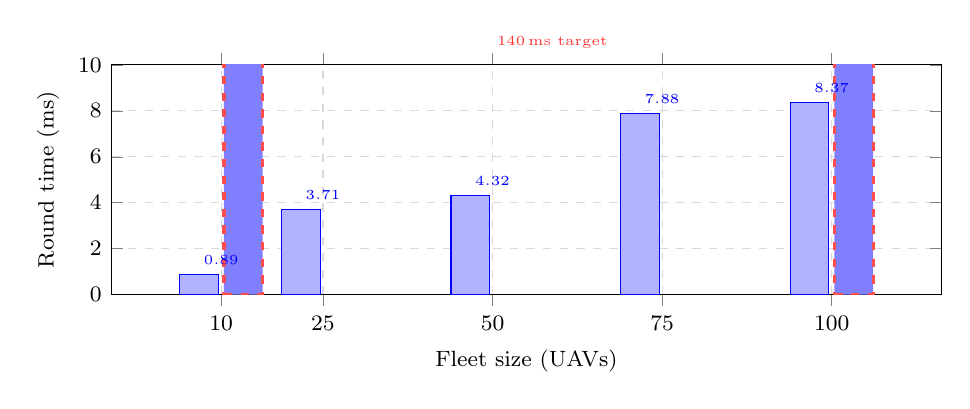
\begin{tikzpicture}
\begin{axis}[
  width=\columnwidth, height=4.5cm,
  xlabel={Fleet size (UAVs)},
  ylabel={Round time (ms)},
  ybar, bar width=14pt,
  xtick={10,25,50,75,100},
  ytick={0,2,4,6,8,10},
  ymin=0, ymax=10,
  enlarge x limits=0.18,
  every axis plot/.append style={fill=blue!50, draw=blue!80},
  nodes near coords, nodes near coords align={vertical},
  every node near coord/.style={font=\tiny},
  grid=major, grid style={dashed,gray!30},
  label style={font=\footnotesize},
  tick label style={font=\footnotesize},
]
\addplot coordinates {(10,0.89) (25,3.71) (50,4.32) (75,7.88) (100,8.37)};
\addplot[draw=red!70, very thick, no marks,
         domain=10:100, samples=4,
         dashed]
  coordinates {(10,140)(100,140)};
\end{axis}
\node[font=\tiny, text=red!80] at (5.6,3.2) {140\,ms target};
\end{tikzpicture}
\caption{DCS round time vs.\ fleet size. All values are $\geq16\times$ below
  the 140\,ms target (dashed red line).}
\label{fig:dcs}
\end{figure}

\begin{table}[t]
\caption{DCS scalability results.}
\label{tab:dcs}
\small
\begin{tabular}{@{}rrrr@{}}
\toprule
\textbf{UAVs} & \textbf{Round time} & \textbf{Target} & \textbf{Margin} \\
\midrule
10  & 0.89\,ms & \textless140\,ms & $157\times$ below \\
25  & 3.71\,ms & \textless140\,ms & $37.7\times$ below \\
50  & 4.32\,ms & \textless140\,ms & $32.4\times$ below \\
75  & 7.88\,ms & \textless140\,ms & $17.8\times$ below \\
100 & 8.37\,ms & \textless140\,ms & $16.7\times$ below \\
\bottomrule
\end{tabular}
\end{table}

\subsection{Security Test Results}

All ten adversarial test cases pass (TC-SEC-01 to TC-SEC-10):
prescription replay (TC-01), unregistered actor (TC-02), revoked HP (TC-03),
fake UAV Bloom/ECDSA (TC-04), wrong patient confirmation (TC-05),
consent-bypassed write (TC-06), TA hijack attempt (TC-07),
direct oracle hash injection (TC-08), wrong DS closing round (TC-09),
and rogue warehouse (TC-10).
Zero false negatives were observed: no legitimate transaction was incorrectly
rejected across the full 86-test suite.

%%====================================================================
\section{Discussion}\label{sec:discussion}
%%====================================================================

\paragraph{Caliper TPS Context.}
The 4.4--4.6 invoke TPS reported in Table~\ref{tab:caliper} reflects
a \emph{single-ordering-node Raft prototype} deployed for functional
validation.
This figure should not be interpreted as the ceiling for production
deployments: Thakkar \etal~\cite{thakkar2018fabric} achieved 3,500\,TPS on
optimised Fabric 1.1, and the Hyperledger Foundation's official Fabric 2.5
Caliper results demonstrate stable low-latency operation at substantially
higher rates with parallelised endorsement and CouchDB caching.
Our result validates that \dcba's chaincode logic is functionally correct
and produces zero transaction failures; throughput optimisation under
multi-node Raft is a planned extension.

\paragraph{DCS Timing Scope.}
The 8.37\,ms DCS figure measures the \emph{score computation phase}
(Python threading for 100 concurrent agents) and the argmax selection.
It does not include network round-trip time for score submission to the
blockchain or Fabric commit latency, which would add Caliper-class latency
per submission.
A complete on-chain DCS round with 100 UAVs submitting in parallel would
see latency dominated by Fabric's commit pipeline; the computation phase
remains 8.37\,ms regardless.

\paragraph{PARS Score Integrity.}
Equation~\eqref{eq:pars} formalises PARS score calculation; however,
the current implementation delegates score entry to the HP without
automated validation.
The RA anomaly-detection mechanism provides post-hoc integrity, but
real-time pre-submission validation — for example, an AI classifier that
cross-references ICD-10 codes against known urgency profiles — would
strengthen pre-entry integrity. This is identified as future work.

\paragraph{Oracle Centralisation.}
The single-relay SC-7 oracle creates a single point of failure in the
cross-chain path. A threshold-signature oracle network (e.g., 3-of-5
independent nodes) would eliminate this risk; implementation is left for
future work.

%%====================================================================
\section{Conclusion}\label{sec:conclusion}
%%====================================================================

We have presented \dcba, a dual-chain blockchain architecture for
secure, priority-aware, UAV-enabled pharmaceutical delivery.
\dcba separates patient data concerns onto an Ethereum PoA PDC and
UAV operational concerns onto a Hyperledger Fabric UOC, connected by a
replay-safe cross-chain oracle.
Six original contributions — dual-chain design, hardware-bound W3C DID,
two-phase DCS algorithm, sanitisable-signature EHR model, \pars clinical
priority routing, and patient-sovereign encryption — collectively address
six confirmed gaps in the prior literature.

Experimental evaluation over 86 automated tests and Hyperledger Caliper
benchmarking demonstrates 100\% security test pass rate, DCS selection in
8.37\,ms for 100-UAV fleets, and zero transaction failures across 244
Caliper transactions.
All ten adversarial attack scenarios are blocked with zero false negatives.
The complete implementation is publicly available at
\url{https://github.com/AnkanSaha18/Blockchain}.

Future work will address oracle decentralisation via a threshold-signature
relay network, adaptive DCS weight optimisation driven by delivery outcome
history, post-quantum migration of ECDSA and ECIES primitives,
and an agent-based Dhaka urban simulation to generate publication-quality
delivery performance figures.

%%====================================================================
\begin{acks}
The authors thank the Department of Computer Science and Engineering at BUET
for providing the computational resources used in this research.
\end{acks}

%%====================================================================
\bibliographystyle{ACM-Reference-Format}
\bibliography{references}

\end{document}
